% !TeX root = ../../main.tex
\section{Introduction}
%he development of a continuous process for the nitration process of toluene into nitrotoluene has been
%A brief introduction to the overall process and a brief description of where reactors appear in the process
This report aims to design a feasible and optimised reactor for the production of o-toluidine, p-aminobenzaldehyde (pABH) and p-aminobenzoic acid (pABA). A total of 4 reactors were commissioned for the overall reaction. 
In particular the nitration reaction of toluene in reactor R101 was selected for rigorous modelling as Nitroma seeks to overcome several major challenges in reactor design including:

\begin{enumerate}
    \item The safety risk of a highly exothermic nitration process of converting toluene into nitrotoluene and to ensure an inherently safer continuous nitration process. 
    \item Transitioning away from a batch process which was mainly used in similar fine chemicals manufacture \cite{di_miceli_raimondi_safety_2015}, into a continuous process. 
    \item Heterogeneous catalysis of the nitration process with the usage of H-Mordenite as opposed to the traditional mixed acid catalyst. 
\end{enumerate}

Reaction kinetics of the nitration of toluene is decided using a combination of literature data and Arrhenius equation. Mathematical modelling including material and energy balances, 2-D concentration and temperature modelling were done on COMSOL 5.6. The reactor was then sized based on British Standard papers and mechanically designed in SolidWorks for visualisation.

%add more stuff for intro 

\subsection{Overview of reactors}
\begin{scheme}[h]
    \centering
    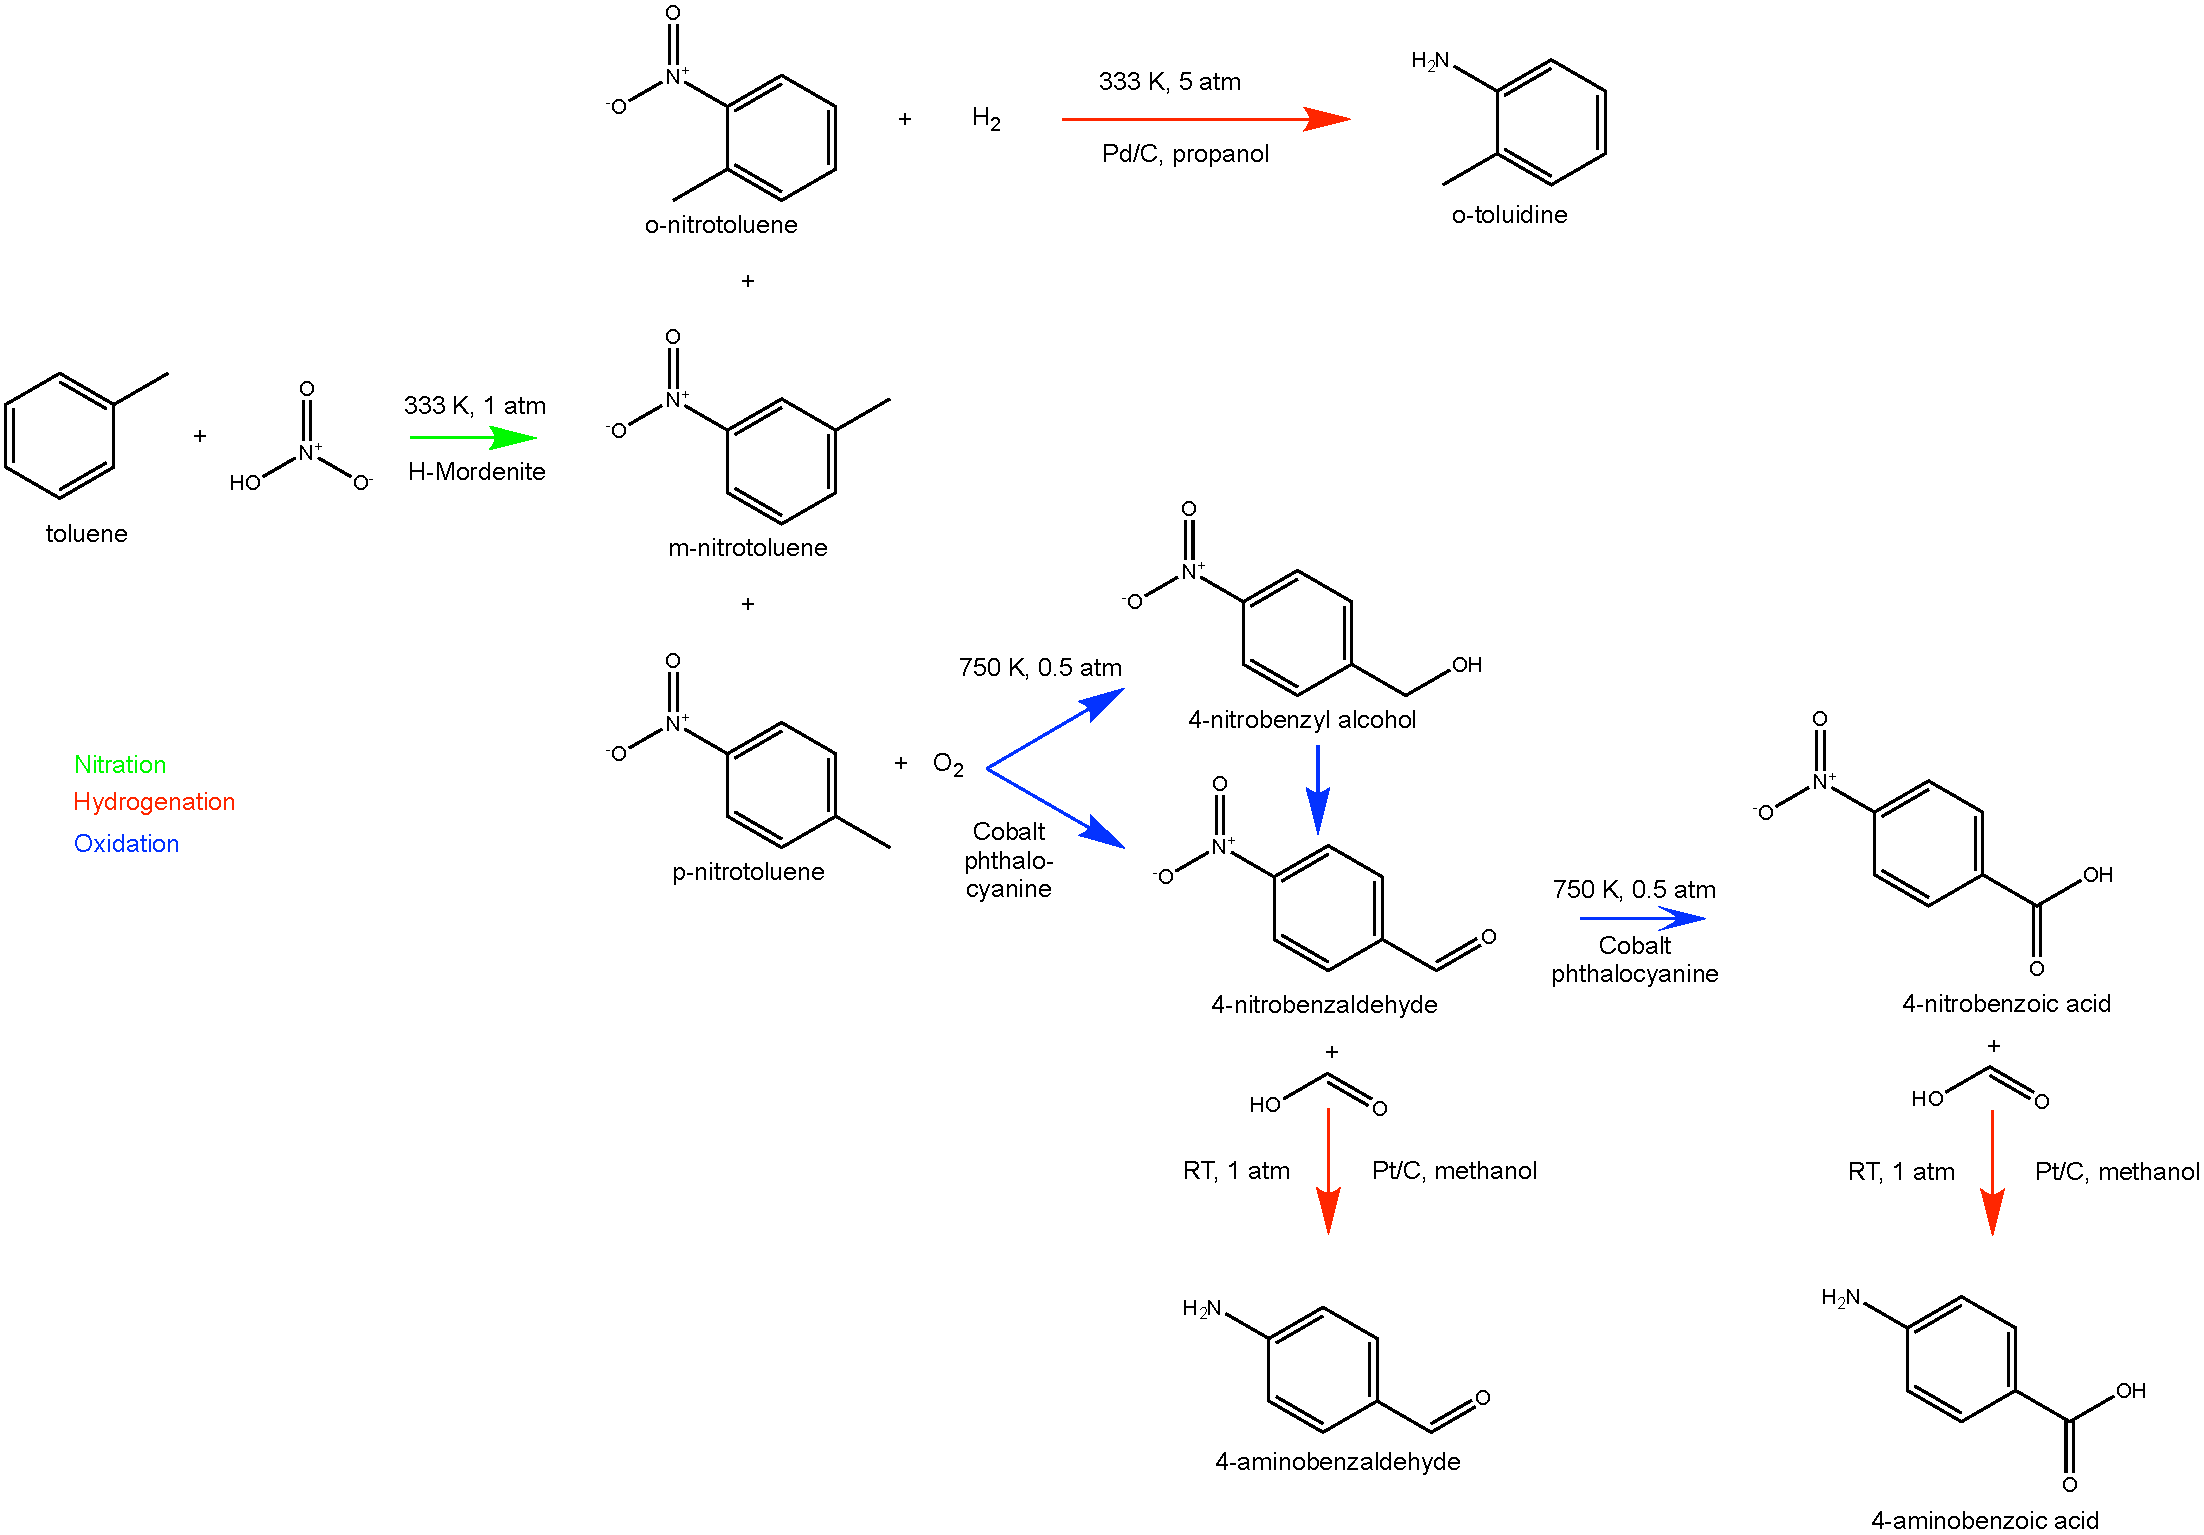
\includegraphics[width=\linewidth]{chapters/2-reaction/figures/routes-chosen.pdf}
    \caption{Overall reaction scheme proposed by Nitroma}
    \label{fig:finalroutes}
\end{scheme}

\Cref{fig:finalroutes} shows the proposed overall reaction scheme of Nitroma's process. The first reactor R101 is an intensified shell-and-tube heat exchanger reactor, used for the nitration of toluene to produce isomers ortho-nitrotoluene (ONT), meta-nitrotoluene (MNT) and para-nitrotoluene (PNT). Next, reactor R201 is a co-current trickle bed reactor that enables the ONT to be hydrogenated into o-toluidine in methanol solvent. Packed-bed reactors R301 and R401 are used for the oxidation of PNT into p-nitrobenzaldehyde (pNBH) and p-nitrobenzoic acid (pNBA) production respectively. Finally, both pNBH and pNBA are hydrogenated into p-aminobenzaldehyde (pABH) and p-aminobenzoic acid (pABA) in packed-bed reactors R501 and R601 respectively. Further details on how each reactors were chosen are detailed in Section \ref{Non-detailed}. 

%Things to double check!
%-sequence of subsections (group by dimension/heat transfer mass transfer?)
%-storyline of reactor? what final KPI should we be looking at?



